\documentclass[twocolumn]{article}

\usepackage[utf8]{inputenc} % allow utf-8 input
\usepackage[T1]{fontenc}    % use 8-bit T1 fonts
\usepackage[hidelinks]{hyperref}       % hyperlinks
\usepackage{url}            % simple URL typesetting
\usepackage{booktabs}       % professional-quality tables
\usepackage{amsmath,amssymb,amsthm}
\usepackage{amsfonts}       % blackboard math symbols
\usepackage{enumitem}
\usepackage{fancyhdr}
\usepackage{float}
\usepackage[a4paper,margin=1in,left=0.7in,right=0.7in]{geometry}
\usepackage{nicefrac}       % compact symbols for 1/2, etc.
\usepackage{makecell}
\usepackage{microtype}      % microtypography
\usepackage{mathrsfs}
\usepackage{graphicx}
\usepackage{doi}
\usepackage{acronym}
\usepackage{listings}
\usepackage{svg}
\usepackage{tikz}
\usepackage[dvipsnames]{xcolor}

\newcommand{\R}{\mathbb{R}}

\fancyhead[LO]{Jonas Pleyer}
\fancyhead[RO]{10/2025}
\fancyhead[CO]{A Cost Function to estimate Parameters of Rod-shaped Bacterial Models}

\begin{document}
\pagestyle{fancy}

\section{Rod-shaped Bacteria}
Rod-shaped bacteria are ubiqitous in nature.
Many mathematical models exist to describe the dynamics of flexible or rigid rods.
One major problem of these tools is that it is difficult to properly estimate their parameters.
We have previously developed methods that are able to estimate the parameters of rod-shaped
bacterial models by comparing them to microscopic images~\cite{Pleyer2025,Pleyer2025_2}.
We extend this work by diving deeper into its mathematical details and establish a mathematical
formulation based on abstractions developed in \cite{Pleyer2025_3}.

\section{Mathematical Model}
We represent bacteria by a collection of vertices $\vec{x}_i\in\R^d$ (with $d=2,3$).
Their dynamics capture effects such as rigidity of the rod, growth, division and physical forces
(see Figure~\ref{fig:mechanics-division}).
Every cell is unique and as a result has a unique identifier $\iota$ assigned to it.
With this identifier we are able to track the relation of mother to daughter cells
which will become important for the parameter estimation later.

\begin{figure}[H]
    \centering
    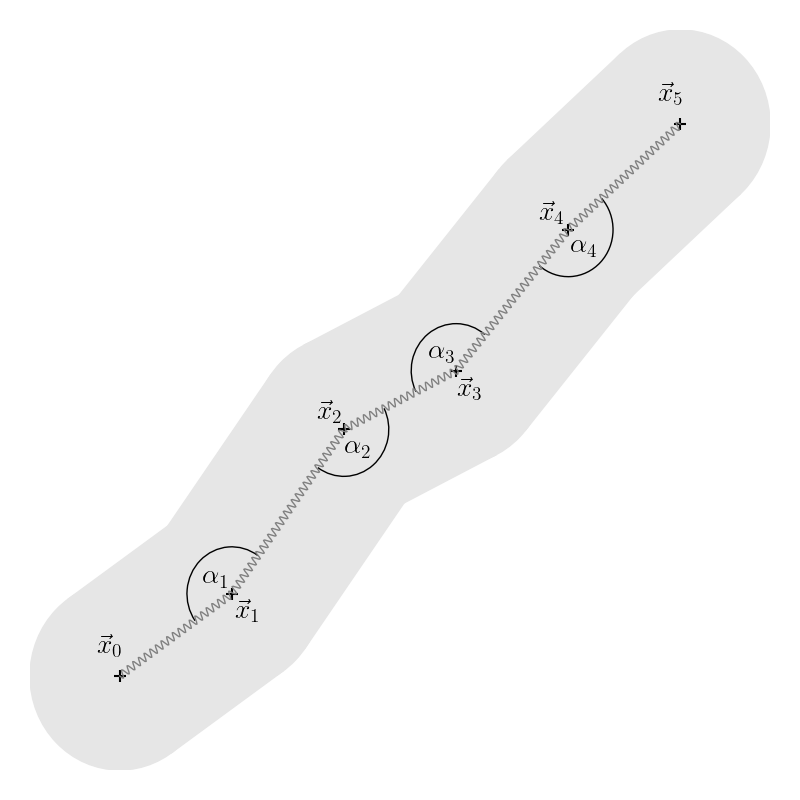
\includegraphics[width=0.4\columnwidth]{figures/mechanics.png}%
    \includesvg[width=0.3\columnwidth]{figures/division.svg}
    \caption{
        (A) A cell which is represented by a collection of vertices.
        (B) A single mother cell divides into two daughter cells.
    }
    \label{fig:mechanics-division}
\end{figure}

\section{Parameter Estimation}
We use microscopic images and obtain their cell masks which serve as datapoints for model comparison.
We are also able to obtain the vertices of the cells $\vec{x}_i$ from them.
In the event that no division occurs, we can directly compare the vertices of one cell
with the experimental data with a least squares approach.
This procedure is performant and effective but can not be applied in the event of a division process.
Due to differing division times, a cell which is present in the simulation might not yet have a
corresponding cell in the experimental data at this time point yet (or vice-versa).
In order to still be able to compare these datapoints, we generate cell-masks as shown in
figure~\ref{fig:cell-masks-comparison}, utilizing the positions within our computational model.
We then compare them to experimental cell-masks by comparing individual pixels and counting every
differing values.
If two color values are related by a mother-daughter relation, we reduce their summation value and
use a "parent-penalty" $0\leq p\leq 1$.
The sum of all pixels is then our cost function.

\begin{figure}
    \centering
    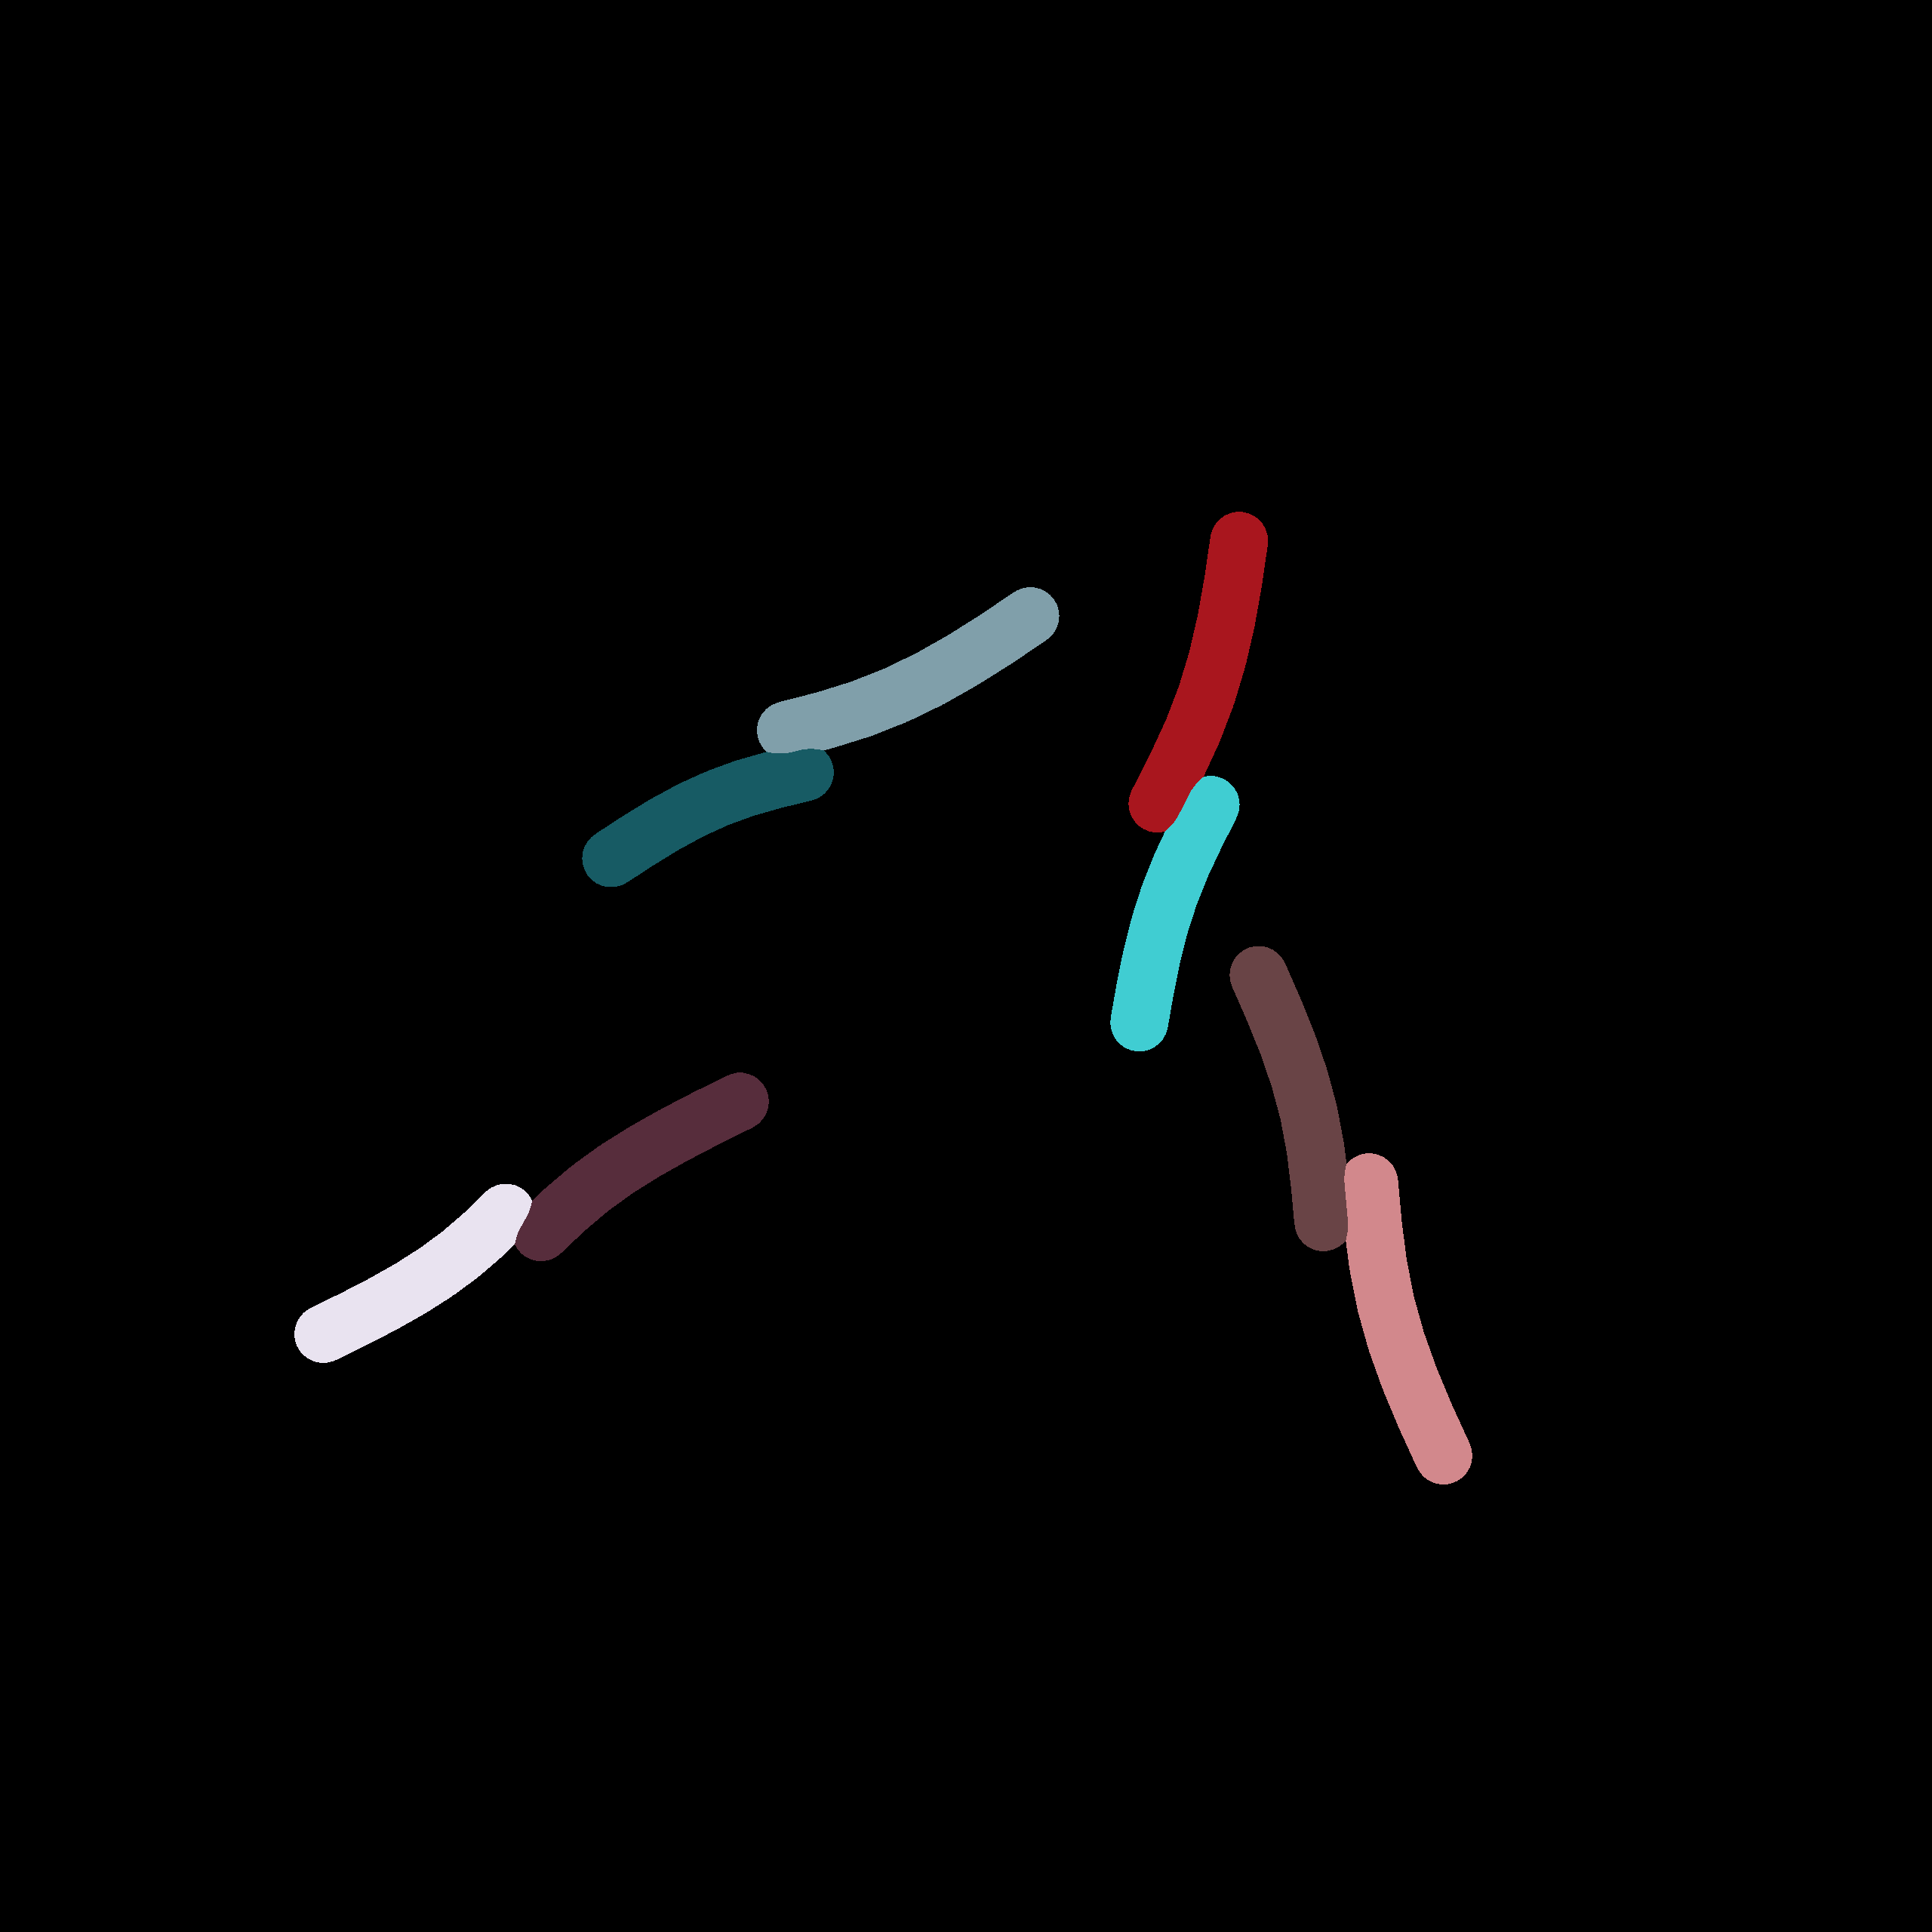
\includegraphics[width=0.4\columnwidth]{figures/progressions-1.png}%
    \hspace{0.01\columnwidth}%
    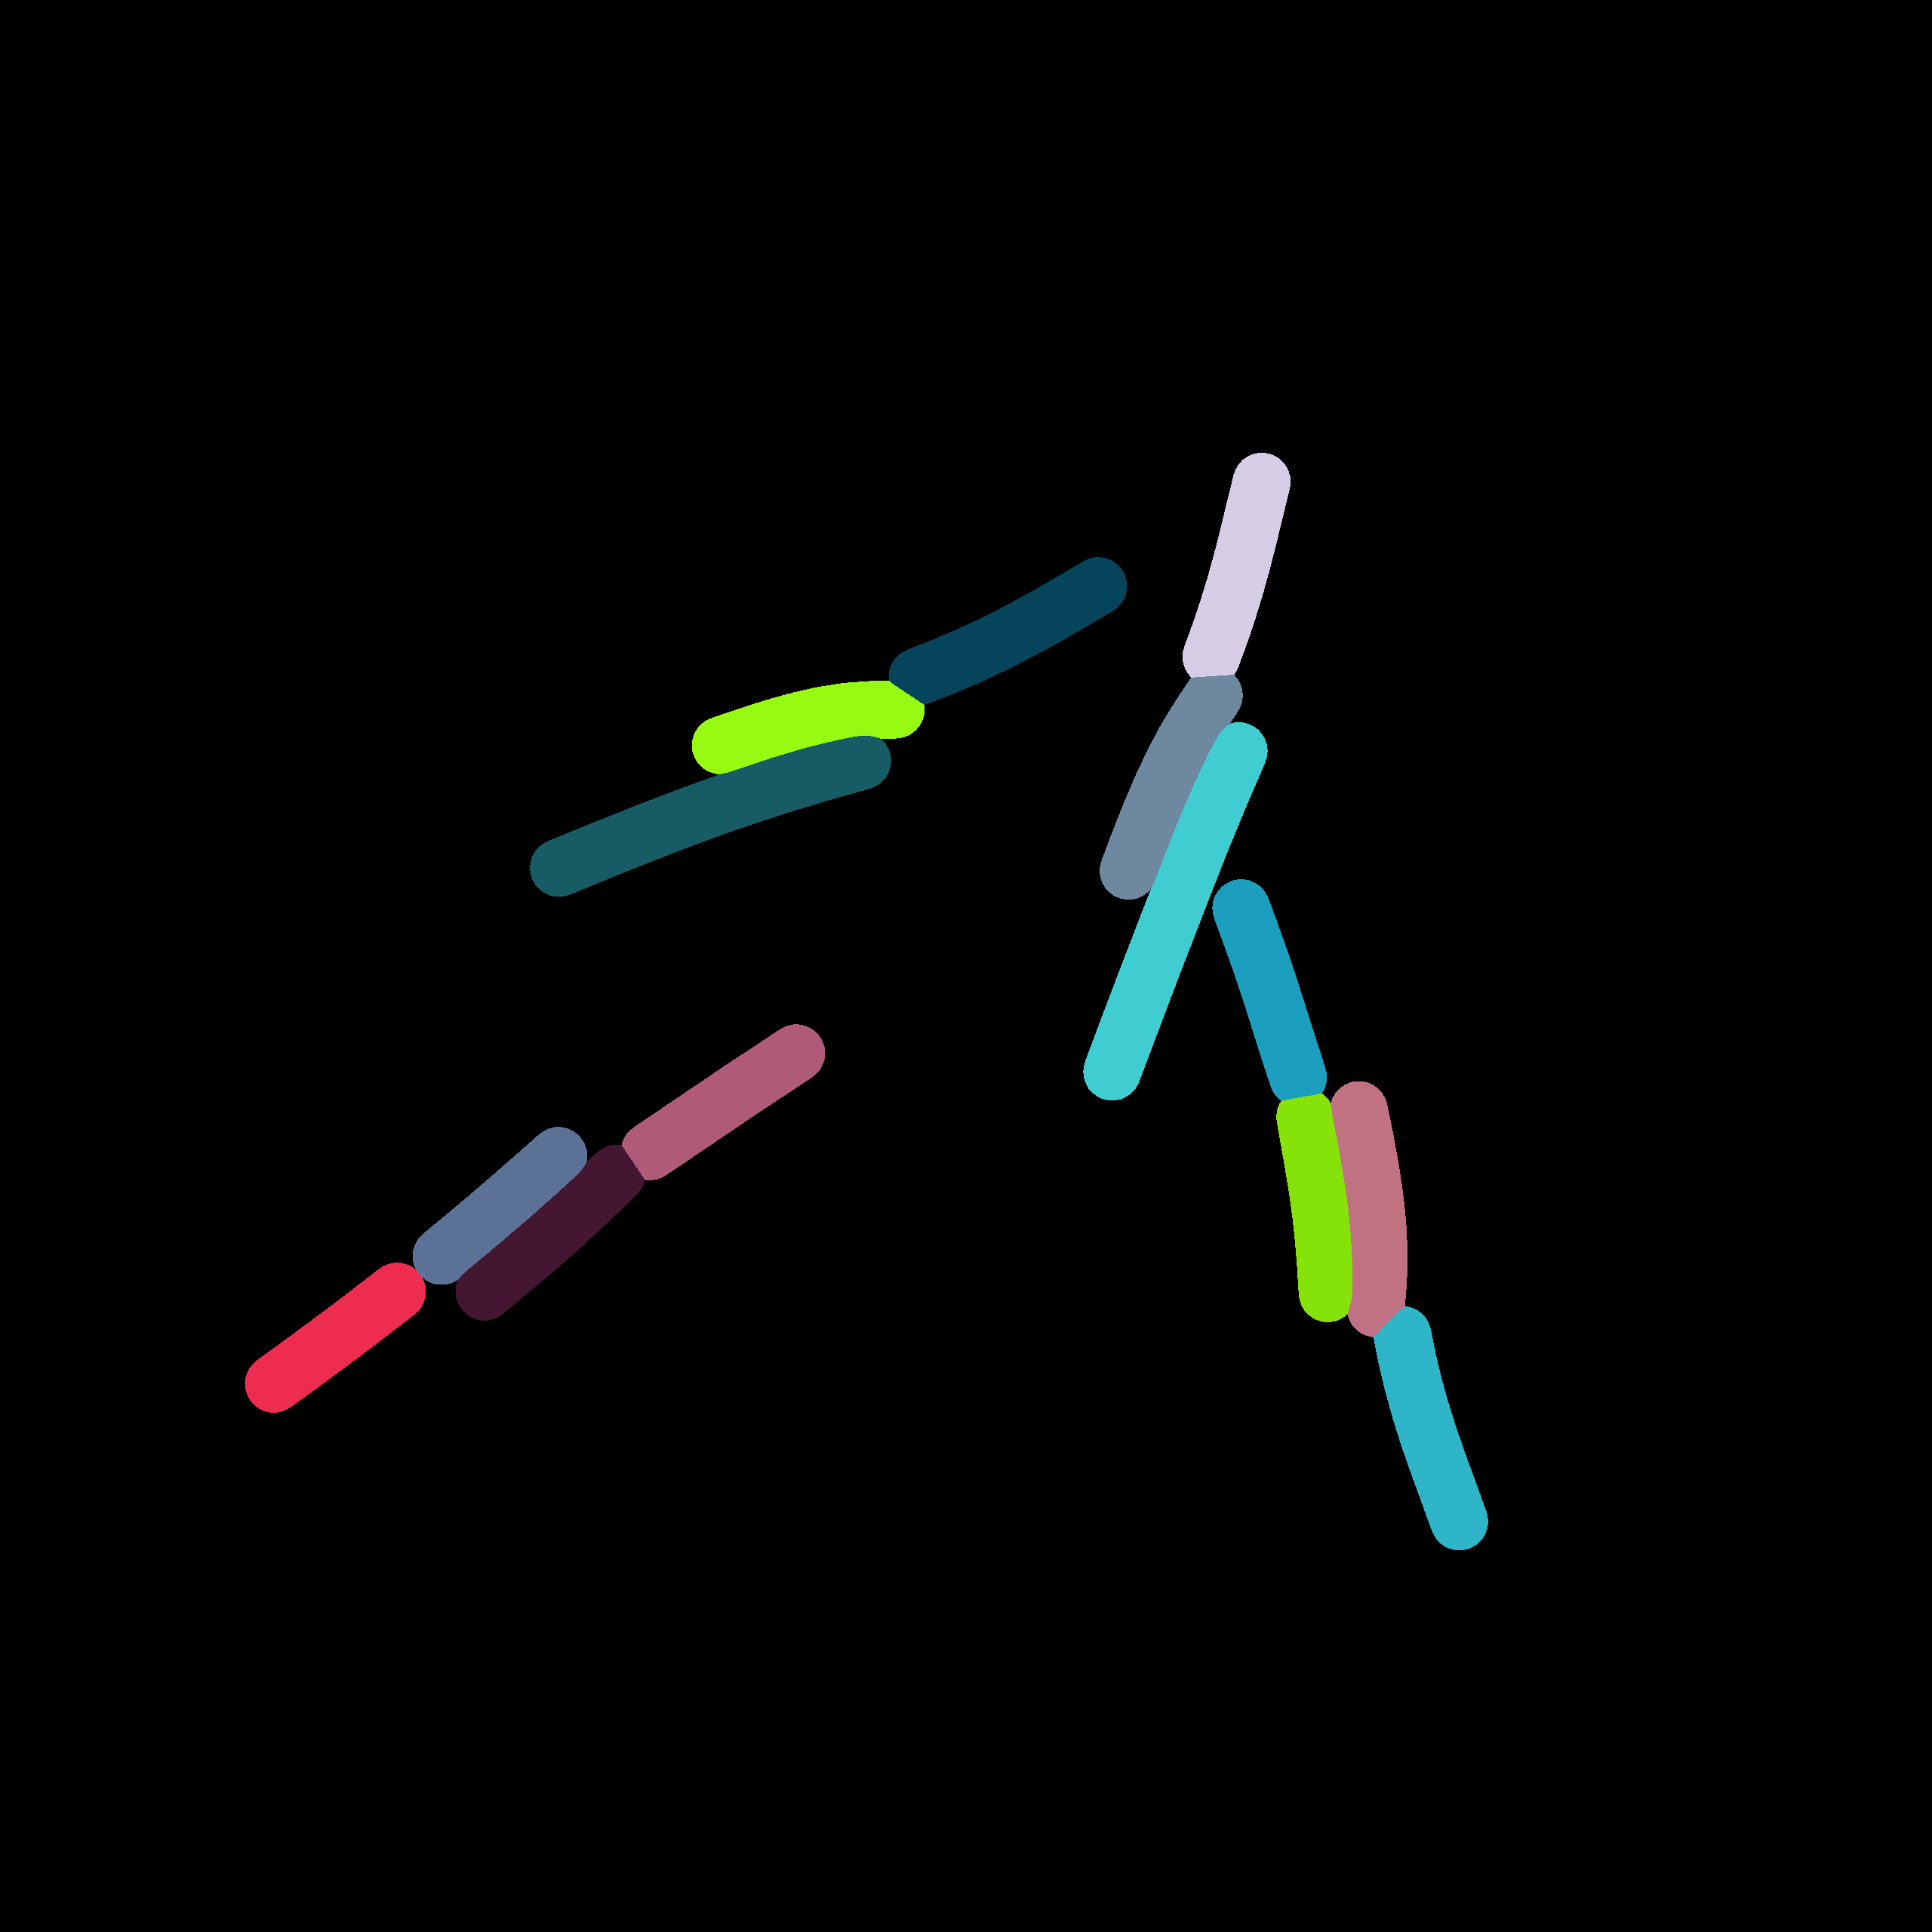
\includegraphics[width=0.4\columnwidth]{figures/progressions-2.png}%
    \hspace{0.01\columnwidth}%
    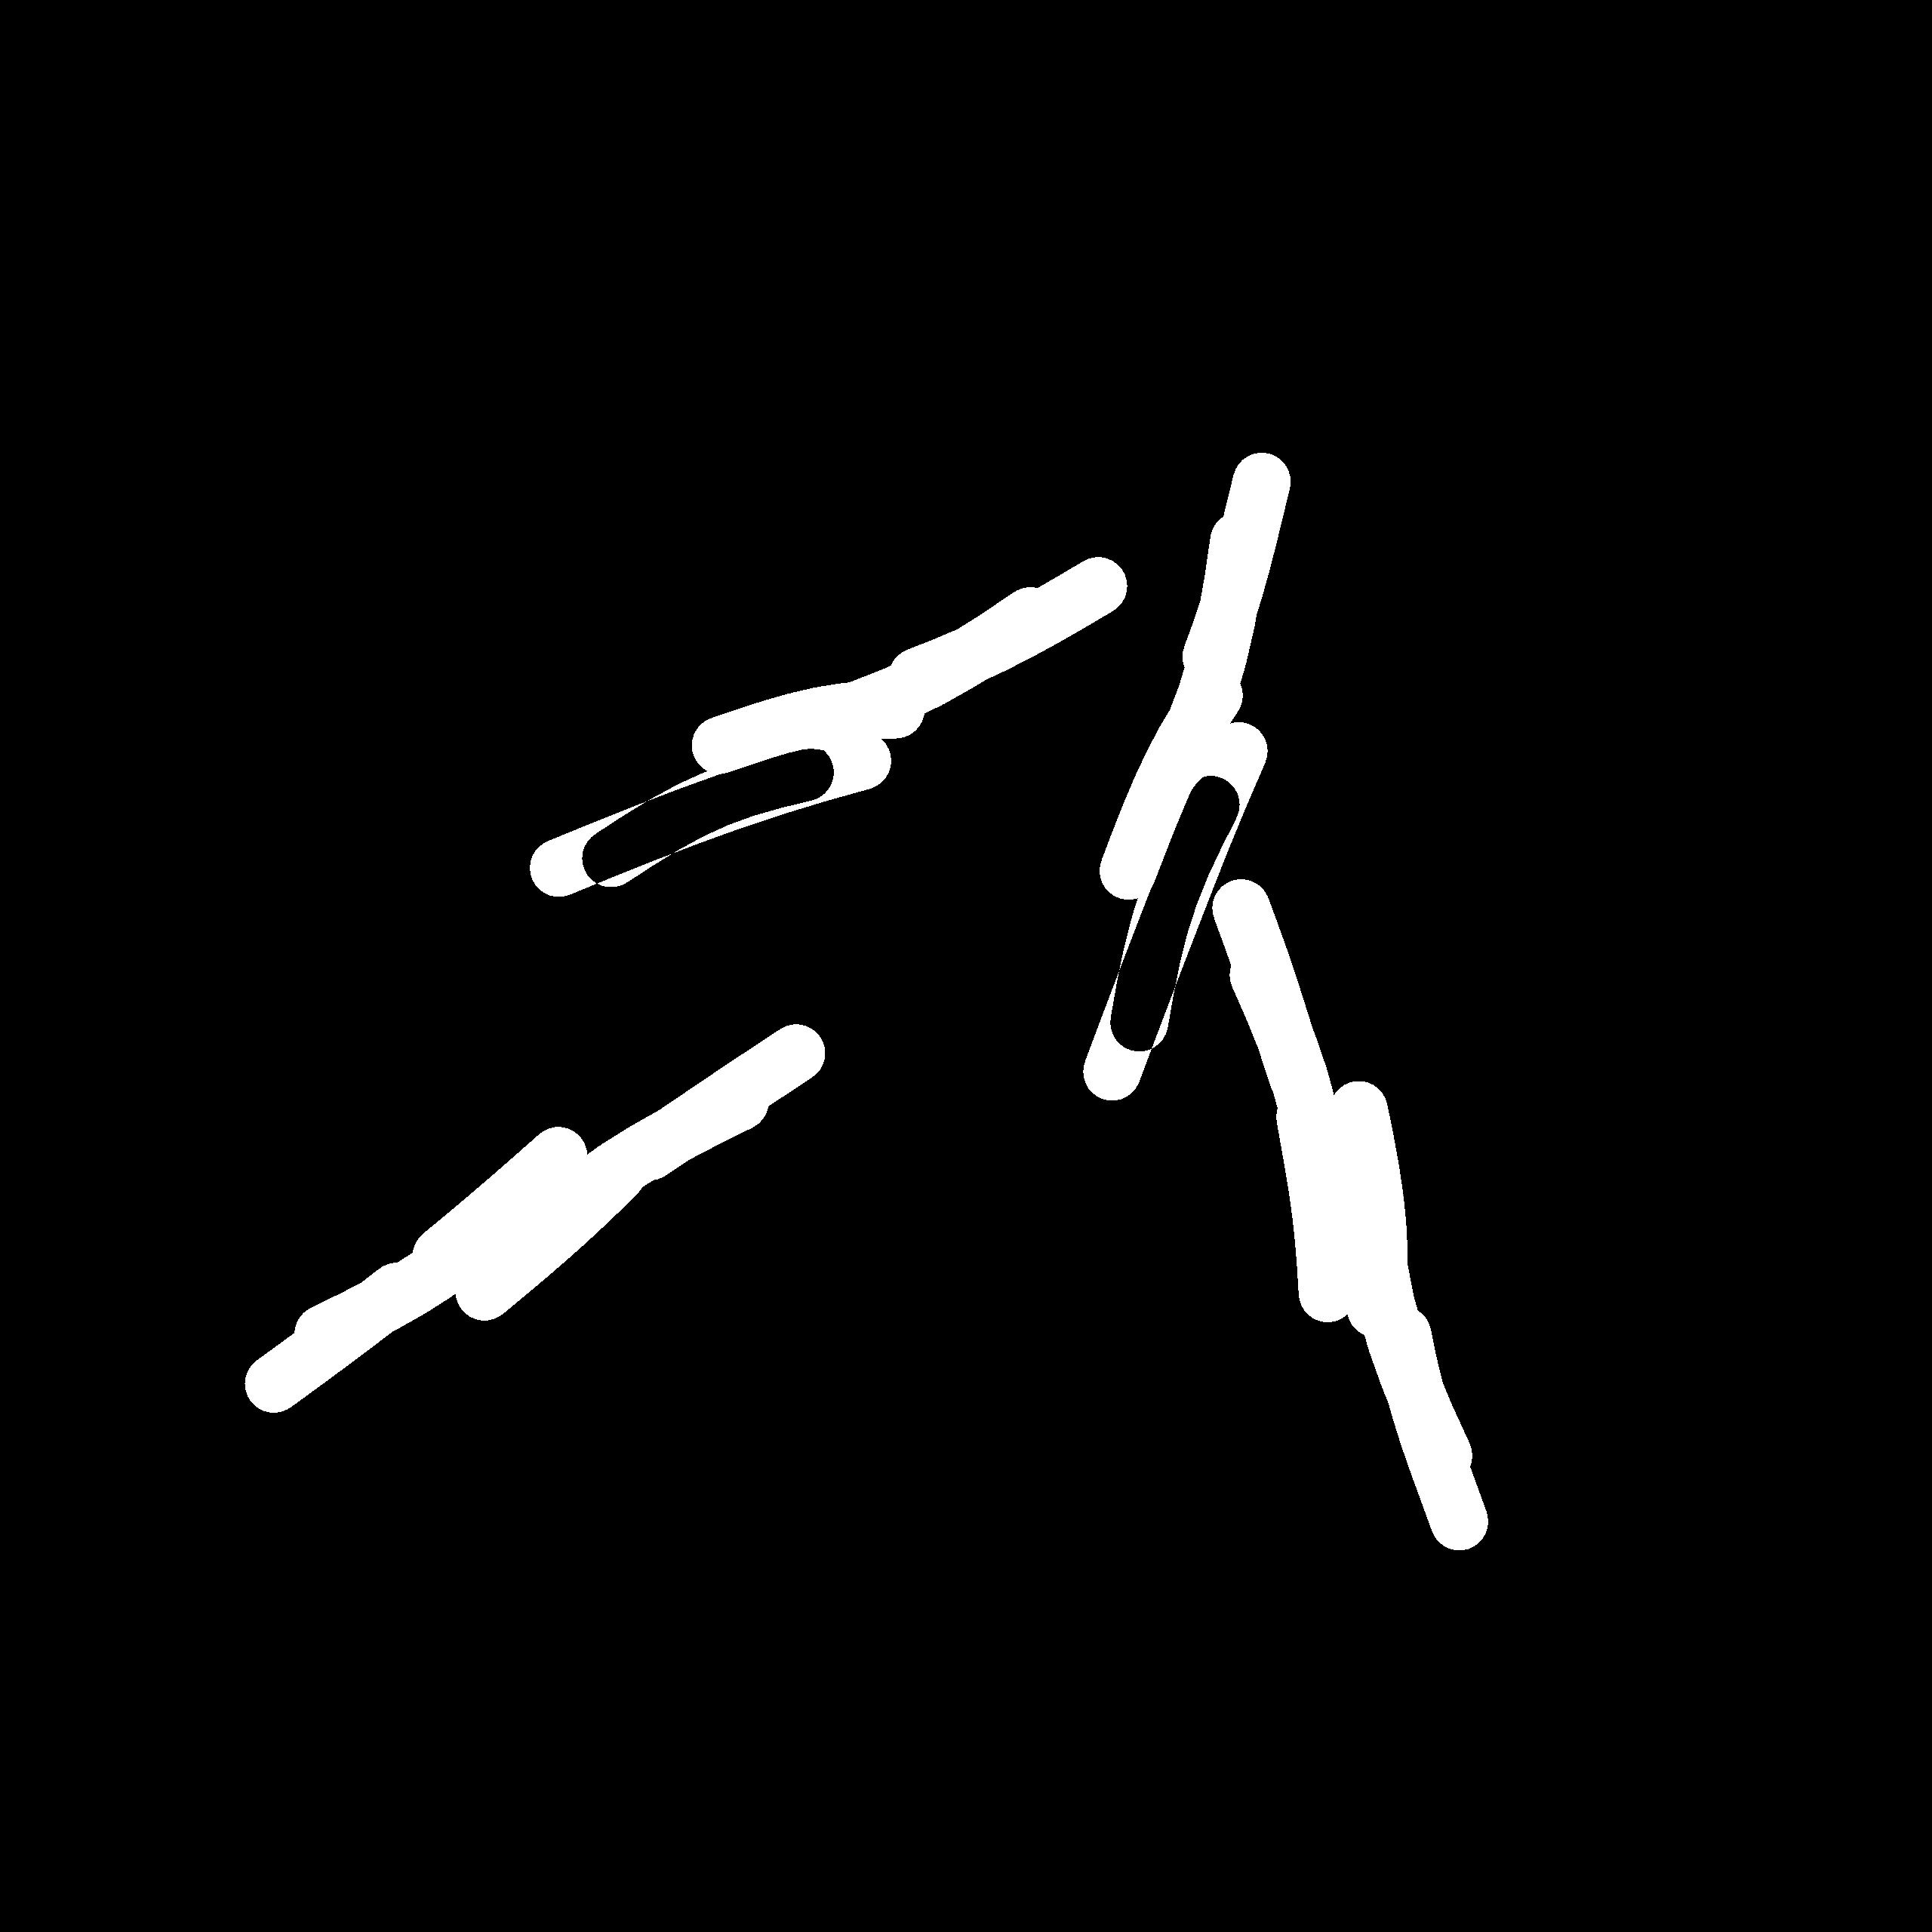
\includegraphics[width=0.4\columnwidth]{figures/progressions-3.png}%
    \hspace{0.01\columnwidth}%
    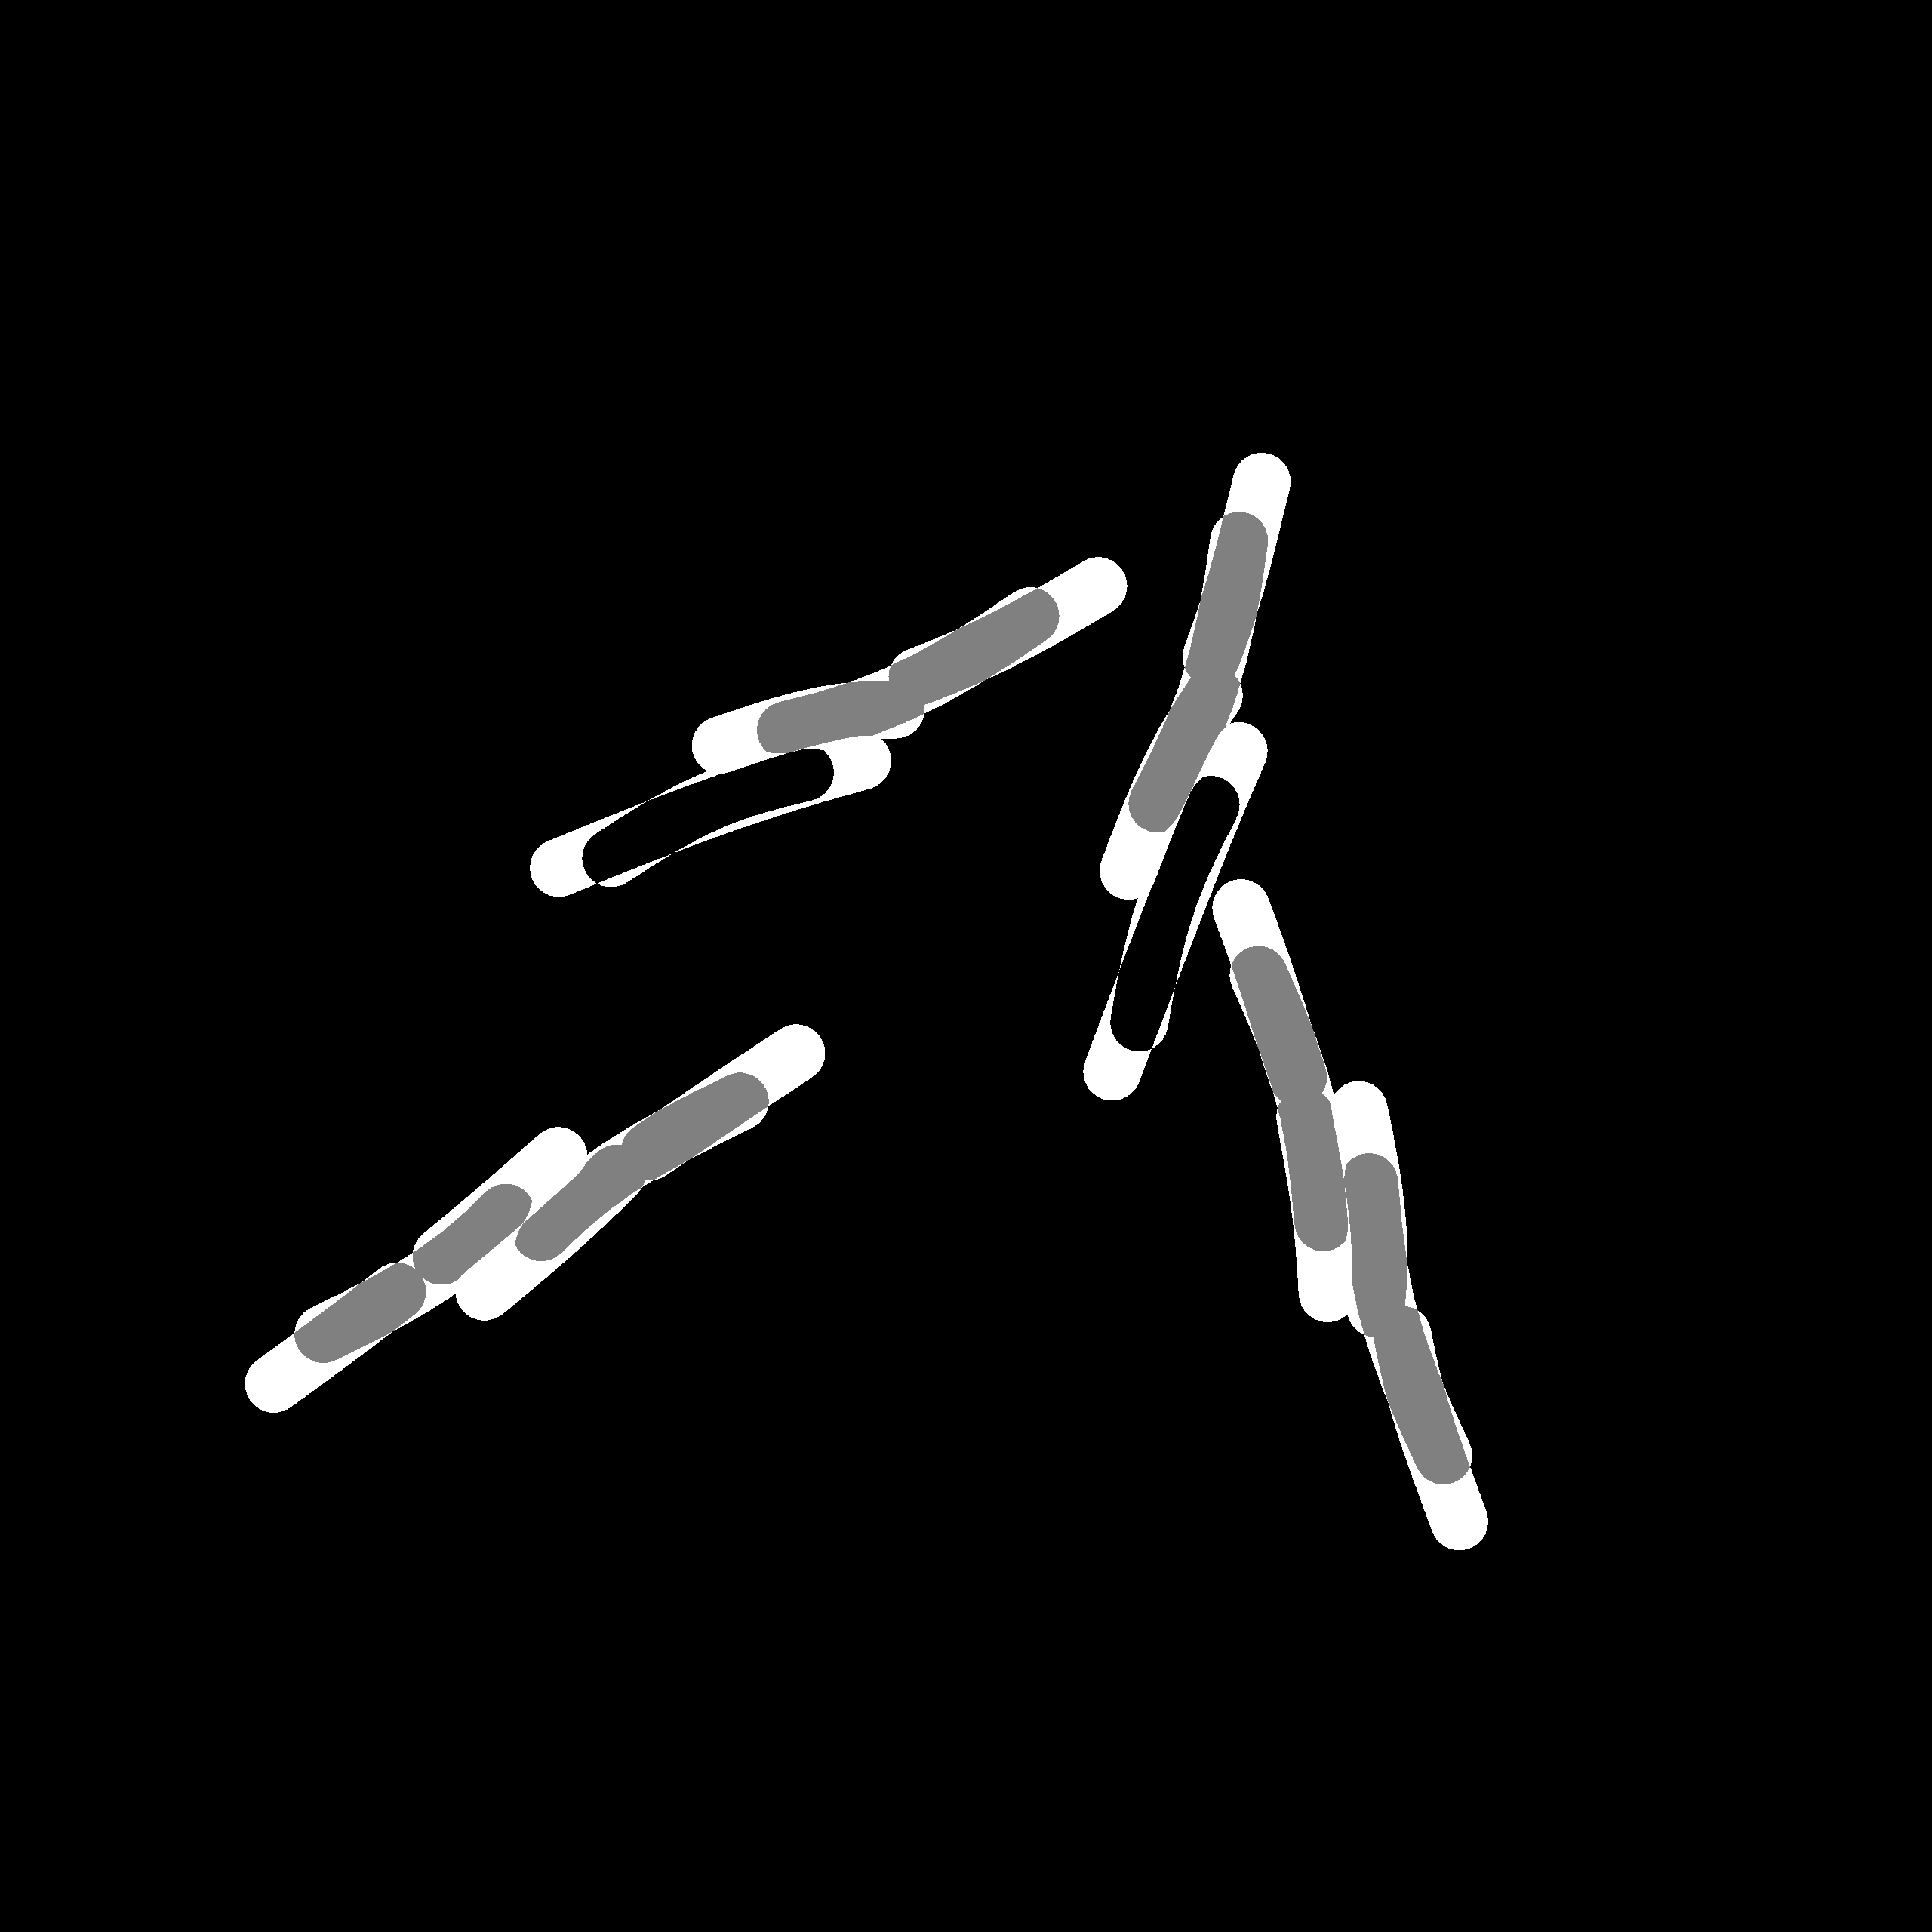
\includegraphics[width=0.4\columnwidth]{figures/progressions-4.png}%
    \caption{
        (A, B) Cell masks that should be compared to each other.
        (C) Difference in pixels.
        (D) Gray areas account for mother-daughter relationship.
    }
    \label{fig:cell-masks-comparison}
\end{figure}

\section{Project}
The goal of this project is to mathematically formalize the previously established methods.
To use this cost function in an optimization routine, it desirable to find a way of efficiently
calculating its derivative.
\begin{enumerate}[noitemsep]
    \item Formalize the notations of these cost functions within our developed theoretical framework
    \item Formulate area comparison with a suitable measure
    \item Add time-dependence to parent-penalty $p=p(t)$.
    \item Discuss how hyperparameters influence results
    \item Show that the area cost function is differentiable with respect to time.
        Or engineer it in such a way that it is (approximatively).
    \item Can we write down an explicit derivative? (that would be hugely benefitial)
    \item Can we use the simpler position comparison algorithm with the area cost function?
    \item Asses possible optimization performance improvements using either of the two previous results
\end{enumerate}

\bibliographystyle{unsrt}
\bibliography{references}

\end{document}
